\subsubsection{Feature Selection and Horizontal Data Reduction}
\label{subsec:feature-selection}

Horizontal data reduction was performed to retain predictors that provide useful information for predicting \textit{Gallstone Status}, while reducing
unnecessary or weakly informative inputs. This was particularly relevant
because the exploratory analysis identified substantial correlation among
several body-composition and laboratory measurements.

\paragraph{Random Forest Feature Importance}
\label{subsubsec:random-forest-importance}

A Random Forest classifier was used as an exploratory feature-ranking method.
Random Forests combine multiple decision trees constructed from bootstrap
samples and random subsets of predictors, allowing nonlinear relationships and
interactions among variables to be captured without requiring strong parametric
assumptions \parencite{breiman2001randomforests}.

Feature importance was calculated using the impurity-based importance measure provided by the RandomForestClassifier implementation in
\texttt{scikit-learn}\footnote{The implementation and definition of
\texttt{feature\_importances\_} are documented in the scikit-learn
\texttt{RandomForestClassifier} API:
\url{https://scikit-learn.org/stable/modules/generated/sklearn.ensemble.RandomForestClassifier.html}.}.

For each predictor, the importance reflects its normalised contribution to the
total reduction in the splitting criterion across the trees in the forest.
The reported values were averaged across the repeated holdout splits, with the
error bars indicating variability in importance across the different random
seeds.

\begin{figure}[H]
    \centering
    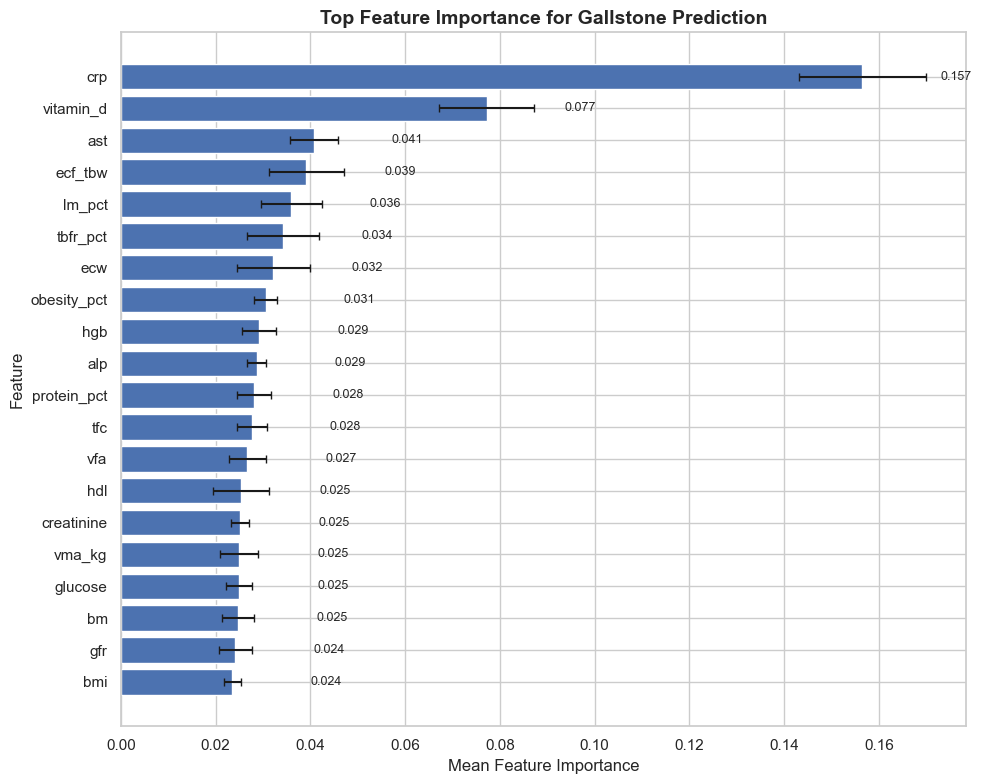
\includegraphics[
        width=0.82\linewidth,
        keepaspectratio
    ]{media/RF_feature_importances.png}
    \caption{Mean Random Forest feature importance for Gallstone Status
    prediction across repeated stratified holdout splits. Error bars represent
    the variability of feature importance across random seeds.}
    \label{fig:random-forest-importance}
\end{figure}

As shown in Figure~\ref{fig:random-forest-importance}, CRP was the most
influential predictor, with a mean importance of approximately 0.157. This was
followed by Vitamin D (0.077), AST (0.041), ECF/TBW (0.039), lean-mass
percentage (0.036), and total body-fat percentage (0.034). ECW,
\texttt{obesity\_pct}, haemoglobin, ALP, protein percentage, total fat content,
VFA, HDL, creatinine, glucose, GFR, and BMI also contributed to the model, but
with smaller individual importance scores.

The ranking suggests that the predictive information is distributed across
multiple clinical domains rather than being dominated by a single type of
measurement. In particular, inflammatory and biochemical variables such as CRP,
AST, and Vitamin D appear alongside body-composition measurements such as
ECF/TBW, lean-mass percentage, total body-fat percentage, ECW, and VFA. This
supports the earlier exploratory findings that Gallstone Status is associated
with a multivariable pattern rather than a simple separation based on one
predictor.

The Random Forest ranking was used as an exploratory assessment of predictor
relevance rather than as the sole criterion for feature removal. Impurity-based
importance can favour variables that provide more potential split points, and
importance values should therefore be interpreted as model-specific indicators
rather than direct measures of clinical effect \parencite{pedregosa2011scikit}.
Final feature-selection decisions were evaluated separately using recursive
feature elimination and predictive performance across the validation
procedures.


\paragraph{Feature Selection After Transformation}
\label{subsubsec:post-transform-selection}

Following the statistical transformation stage, feature selection was performed
using the open-source Python modelling stack. Both the original predictors and
the transformed representations were included as candidate inputs so that the
usefulness of each representation could be evaluated empirically rather than
assuming that transformation would automatically improve prediction.

Horizontal data reduction was performed using Recursive Feature Elimination
(RFE) with a CART decision-tree classifier as the underlying estimator. CART
provides a nonlinear feature-ranking mechanism based on reductions in node
impurity, while RFE recursively removes the least informative predictors and
re-fits the estimator on the remaining feature set. This procedure therefore
reduces the dimensionality of the modelling dataset while retaining variables
that contribute most strongly to the separation of
\textit{Gallstone Present} and \textit{Gallstone Absent} cases.

Feature selection was performed within the training partition for each random
seed to avoid using information from the validation or test data. The resulting
feature rankings were then compared across repeated holdout splits to assess the
stability of the selected predictors.

\begin{figure}[H]
    \centering
    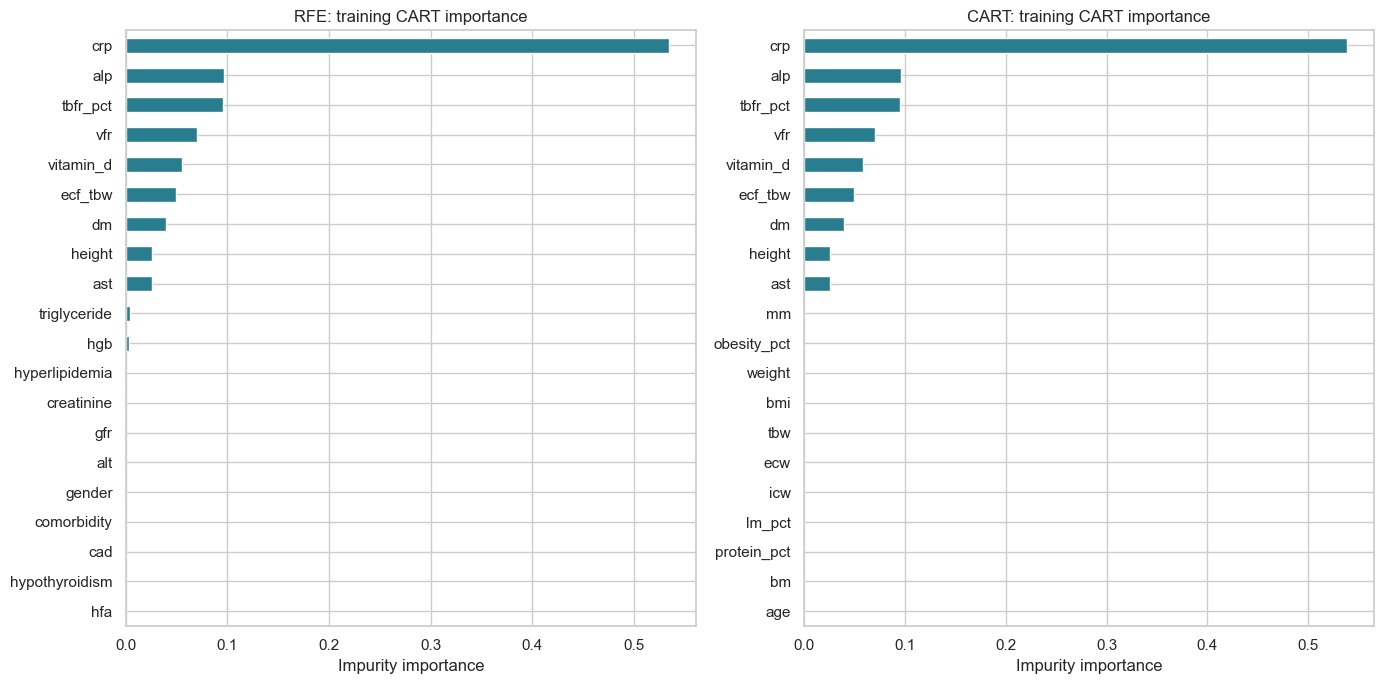
\includegraphics[
        width=0.95\linewidth,
        keepaspectratio
    ]{media/RFE_CART_FE.png}
    \caption{CART-based feature importance used within the recursive feature
    elimination procedure. Predictor importance was estimated using the
    training data only.}
    \label{fig:rfe-cart-importance}
\end{figure}

As shown in Figure~\ref{fig:rfe-cart-importance}, CRP was the dominant predictor
in the CART-based ranking. ALP and total body-fat percentage
(\texttt{tbfr\_pct}) formed the next most influential group, followed by
visceral fat rating (\texttt{vfr}), Vitamin D, ECF/TBW, and diabetes mellitus
(\texttt{dm}). Several additional variables, including height and AST,
contributed more weakly to the fitted tree.

The dominance of CRP was also visible in the individual CART structures. In the
two example training splits shown in Figures~\ref{fig:cart-seed7} and
\ref{fig:cart-seed42}, CRP was selected as the root split, while subsequent
branches incorporated different combinations of body-composition and clinical
variables such as bone mass, ECF/TBW, total body-fat percentage, Vitamin D,
VFR, BMI, and ALP.

\begin{figure}[H]
    \centering
    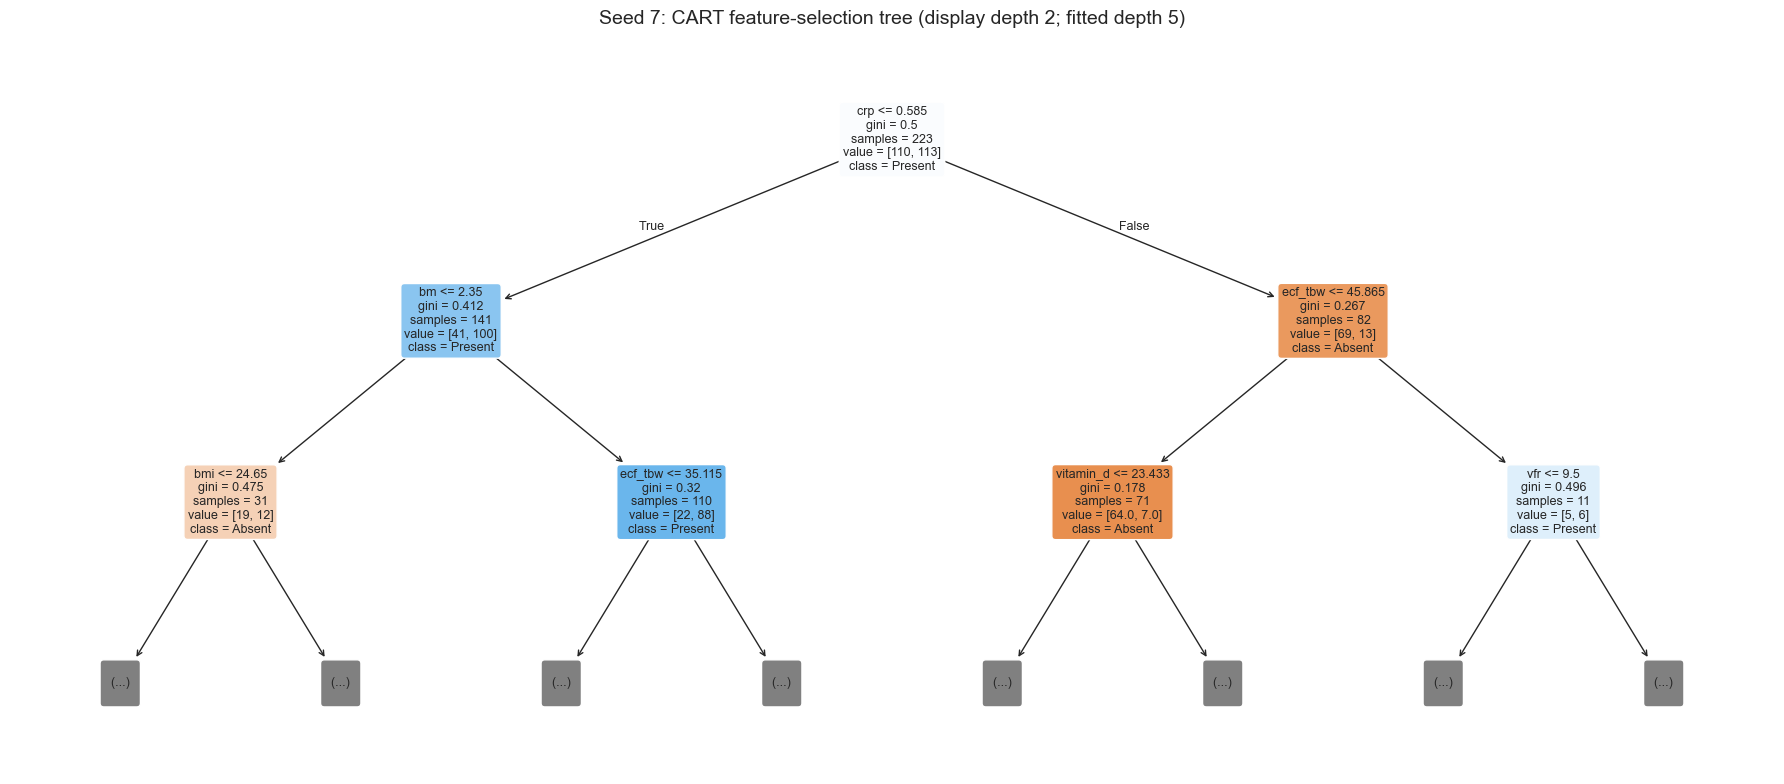
\includegraphics[
        width=\linewidth,
        keepaspectratio
    ]{media/CART_Tree_2.png}
    \caption{Example CART feature-selection tree for one training split. Only
    the upper levels of the fitted tree are displayed for interpretability.}
    \label{fig:cart-seed7}
\end{figure}

\begin{figure}[H]
    \centering
    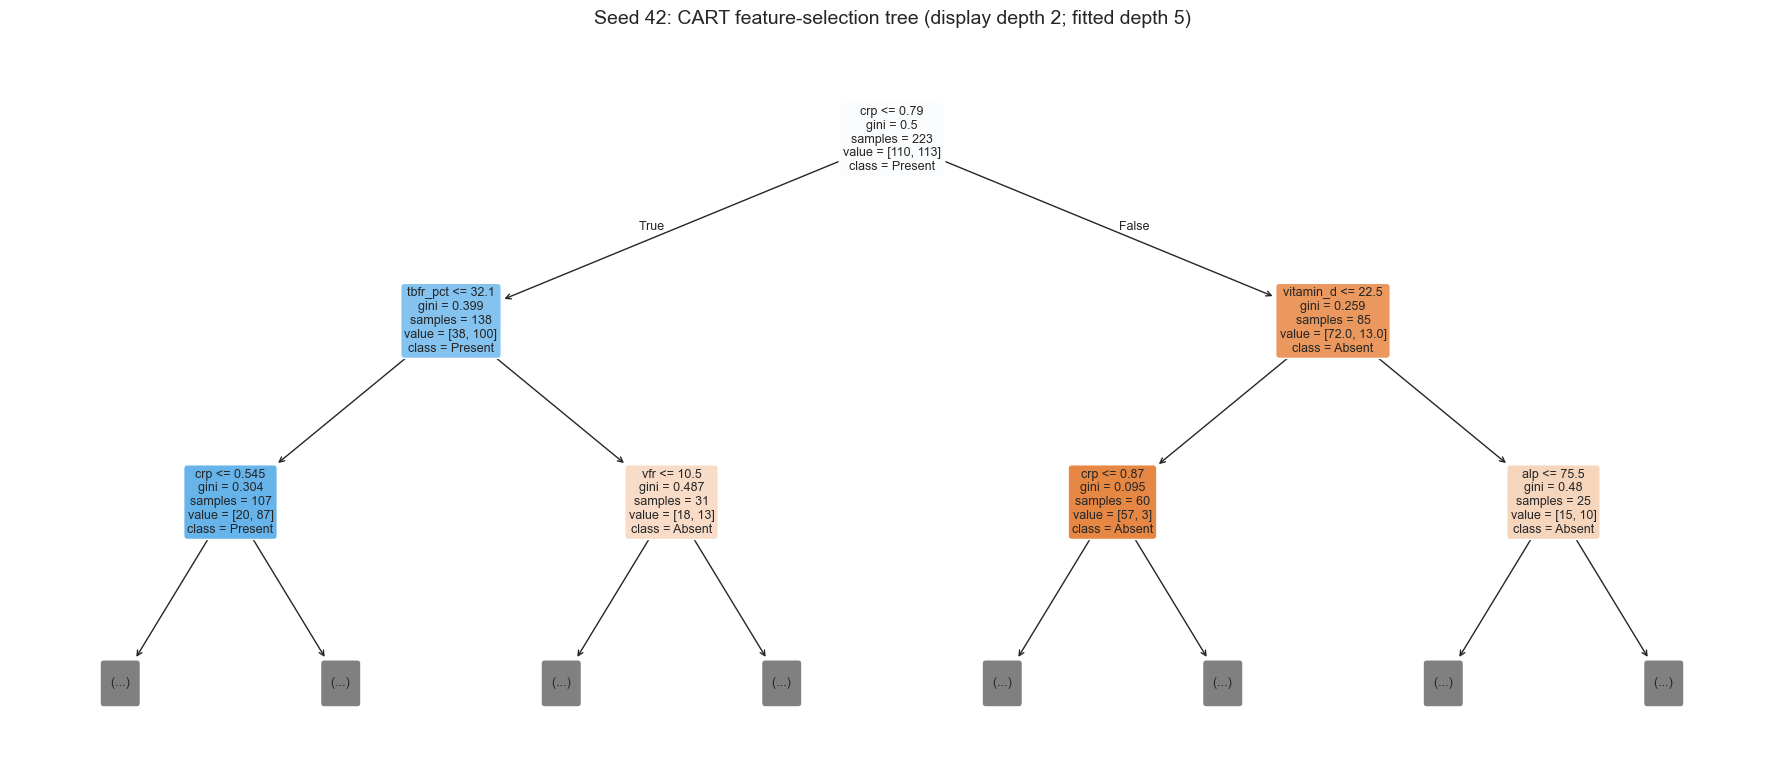
\includegraphics[
        width=\linewidth,
        keepaspectratio
    ]{media/CART_Tree_1.png}
    \caption{Example CART feature-selection tree from a second training split,
    illustrating variation in lower-level splits while retaining CRP as the
    primary separating feature.}
    \label{fig:cart-seed42}
\end{figure}

The variation in the lower branches across training splits indicates that the
dataset does not depend on a single fixed decision rule. Instead, several
clinical and body-composition variables provide complementary information.
Variables appearing repeatedly across the RFE rankings and CART structures were
therefore considered more stable candidates than variables selected only in a
single split.

The final number of predictors was not determined using an arbitrary importance
threshold. Instead, progressively reduced top-$k$ feature subsets generated by
RFE were evaluated on the validation data, and the number of retained features
was selected according to predictive performance across the repeated splits.
This provides a direct link between feature reduction and out-of-sample model
performance.

Together with the preceding transformation stage, this procedure addresses two
forms of data preparation. Statistical transformations project strongly skewed
measurements into alternative numerical representations, while RFE and CART
provide horizontal reduction by removing predictors that contribute limited
additional information. The resulting reduced feature set was subsequently
carried forward to model development and compared with the broader predictor
set.

\paragraph{Vertical Reduction.}
No vertical reduction was applied to the dataset. The available sample contains only 319 observations, so removing records without a clear data-quality reason could unnecessarily reduce the amount of information available for training and evaluation. In addition, the target variable is
already well balanced, with 161 observations representing gallstones present and 158 representing gallstones absent. The exploratory analysis therefore provided no evidence that undersampling or other record-reduction techniques
were required.

All valid observations were consequently retained, while stratified partitioning was used to preserve the target distribution across the
training, validation, and test sets. Data reduction in this project instead
focused on \textit{horizontal reduction}, where feature-selection methods were
used to identify and retain predictors that were most relevant to \textit{Gallstone Status}.

\subsubsection{Statistical Transformation}
\label{subsec:data-transformation}

Exploratory analysis identified substantial skewness in several continuous
predictors, particularly \texttt{obesity\_pct}, ALT, AST, HDL, glucose, CRP,
triglyceride, GFR, and VFA. Rather than transforming all numerical variables,
transformation was considered only for features with
$|\mathrm{skewness}| \geq 1$.

Two transformation approaches were evaluated: the logarithmic transformation
and the Yeo--Johnson power transformation. Their effectiveness was assessed by
comparing the resulting distributions and sample skewness with the original
measurements.

\begin{figure}[H]
    \centering
    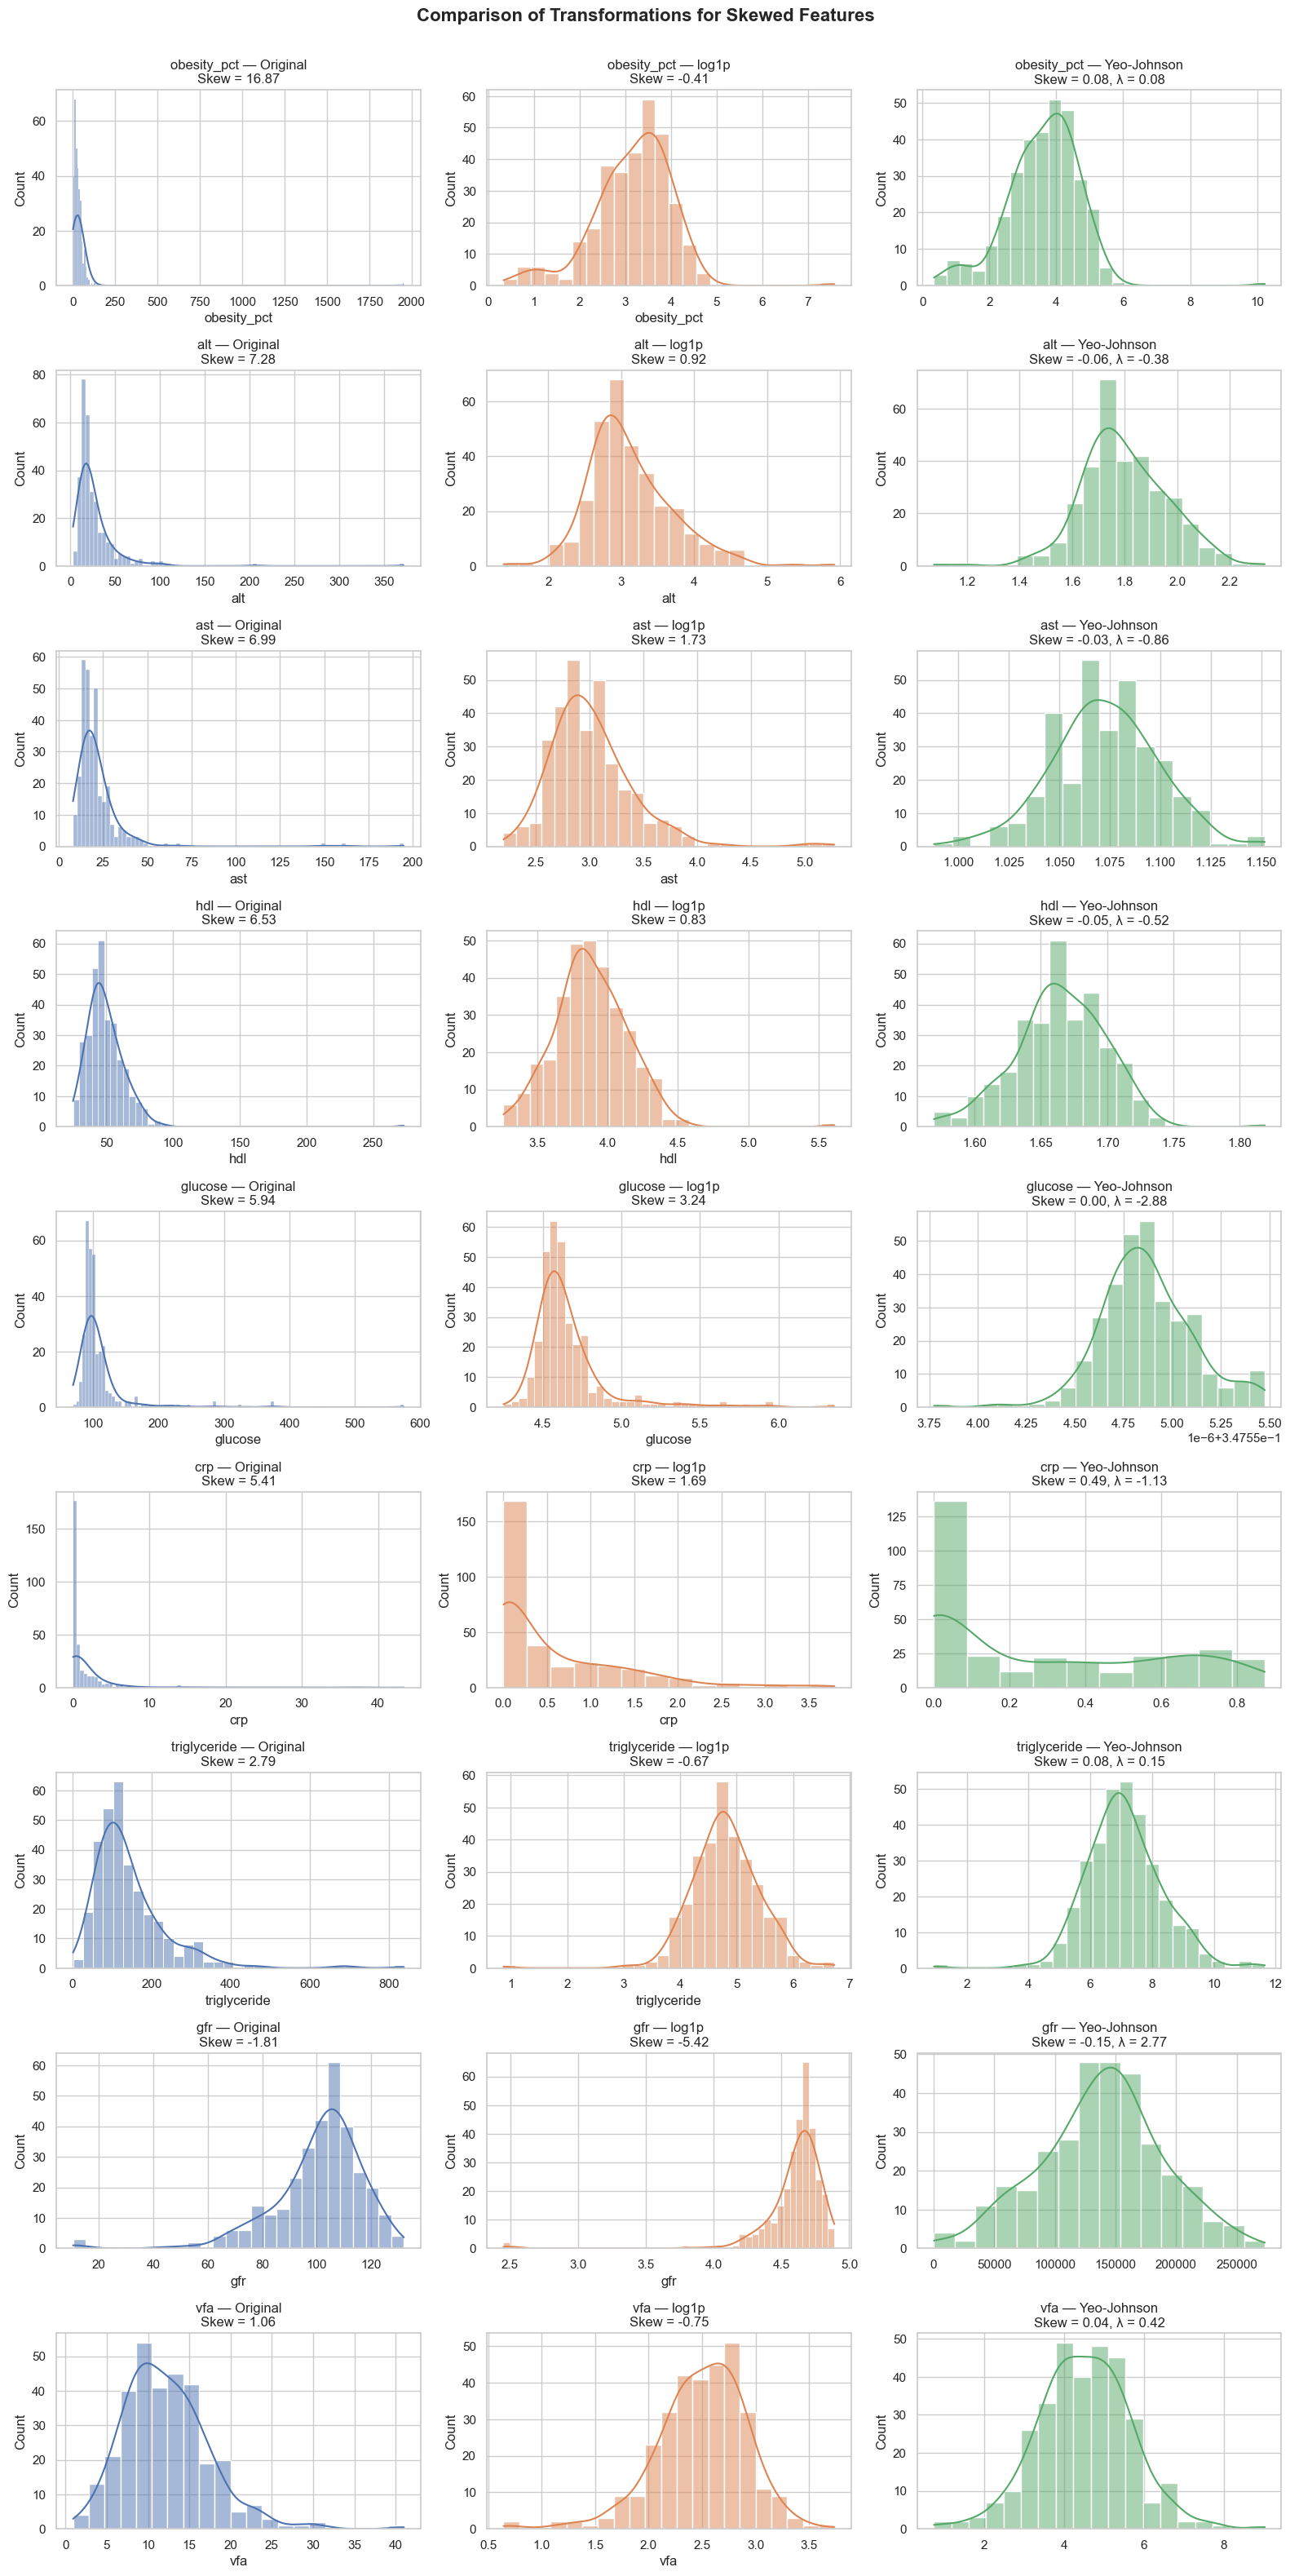
\includegraphics[
        width=\linewidth,
        height=0.88\textheight,
        keepaspectratio
    ]{media/transformation_exetrme.png}
    \caption{Comparison of the original, \texttt{log1p}, and Yeo--Johnson
    distributions for continuous variables with absolute skewness greater than
    or equal to 1. Reported values show the resulting skewness and the estimated
    Yeo--Johnson parameter $\lambda$.}
    \label{fig:transformation-comparison}
\end{figure}


\paragraph{Logarithmic Transformation}
\label{subsubsec:log-transformation}

For non-negative variables, a logarithmic transformation was evaluated using

\[
x_{\mathrm{log}} = \log(1+x),
\]

where the addition of one allows zero-valued observations to be retained.

As shown in Figure~\ref{fig:transformation-comparison}, the transformation
substantially reduced positive skewness for several variables. For example,
the skewness of \texttt{obesity\_pct} decreased from 16.87 to approximately
$-0.41$, while ALT decreased from 7.28 to 0.92 and triglyceride from 2.79 to
0.67. However, the improvement was not consistent across all predictors.
Glucose, for example, remained noticeably right-skewed after transformation,
with skewness decreasing from 5.94 to 3.24.

The logarithmic transformation was therefore treated as a feature-specific
preprocessing option rather than being applied uniformly to all continuous
variables.


\paragraph{Yeo--Johnson Transformation}
\label{subsubsec:yeojohnson-transformation}

The Yeo--Johnson transformation was also evaluated as a more flexible power
transformation. Unlike conventional logarithmic or Box--Cox transformations,
the Yeo--Johnson method can accommodate zero and negative values while
estimating an appropriate transformation parameter, $\lambda$, from the data
\parencite{yeo2000new}.

The transformation is defined piecewise according to the value of $x$ and the
estimated parameter $\lambda$, allowing the shape of the transformation to
adapt to each variable. This makes it particularly useful when continuous
predictors differ substantially in scale and distribution.

Figure~\ref{fig:transformation-comparison} shows that Yeo--Johnson generally
produced stronger reductions in absolute skewness for the most asymmetric
variables. For example, skewness decreased from 16.87 to approximately 0.08
for \texttt{obesity\_pct}, from 7.28 to $-0.06$ for ALT, from 6.99 to 0.03
for AST, and from 5.94 to approximately 0.00 for glucose. Triglyceride was
similarly reduced from 2.79 to approximately 0.08.

These results indicate that Yeo--Johnson provided a more consistent
normalisation of strongly skewed predictors than the logarithmic
transformation for this dataset. Nevertheless, improved symmetry alone was not
used as sufficient justification for retaining a transformed feature.
Transformed and original representations were subsequently evaluated through
feature selection and predictive model performance.


\paragraph{Transformation within the Modelling Pipeline}
\label{subsubsec:transformation-pipeline}

Transformations were implemented as part of the modelling pipeline rather than
as permanent modifications to the source data. Original measurements were
retained for traceability, while transformation parameters were estimated using
the training data only and then applied unchanged to the corresponding
validation and test partitions.

This procedure prevents information from held-out observations from influencing
preprocessing decisions and reduces the risk of data leakage. The final choice
between original and transformed representations was therefore based on both
distributional improvement and downstream predictive performance rather than on
normality alone.

